\documentclass[11pt,bibtotoc,idxtotoc,a4paper,pointlessnumbers]{report}

% allow sophisticated control structures
\usepackage{ifthen}

% use a whole a4 page
\usepackage{a4wide}

% show program code\ldots
\usepackage{verbatim}
%\usepackage{program}

% use colors
\usepackage{color}
\definecolor{darkgreen}{rgb}{0,0.5,0.1}

\usepackage{graphics}

%----------------------------------------------------
%      Graphics and Hyperlinks
%----------------------------------------------------

% check for pdfTeX
\ifx\pdftexversion\undefined
 % use PostScript graphics
 \usepackage[dvips]{graphicx}
 \DeclareGraphicsExtensions{.eps,.epsi}
 % use hypertex version of hyperref
 \usepackage[hypertex,hyperindex=false]{hyperref}
\else
 % reduce output size
 \pdfcompresslevel=9
 % declare pdfinfo
 \pdfinfo {
   /Title (gl-117.pdf)
   /Creator (pdfLaTeX)
   /Author (Thomas A. Drexl)
   /Subject (GL-117 documenation)
   /Keywords (gl-117, flight simulator, documentation)
 }
 % use pdf or jpg graphics
 \usepackage[pdftex]{graphicx}
 \DeclareGraphicsExtensions{.jpg,.png,.pdf}
 % use pdftex version of hyperref
 \usepackage[pdftex,colorlinks=true,linkcolor=blue,citecolor=blue,%
 anchorcolor=darkgreen,urlcolor=darkgreen,bookmarks=true,%
 bookmarksopen=true,bookmarksopenlevel=0,plainpages=false%
 bookmarksnumbered=true,hyperindex=false,pdfstartview=%
 ]{hyperref}
\fi

%-------------------------------------------------------------
%                      Own Commands
%-------------------------------------------------------------

\newcommand {\bsl} {$\backslash$}

\newcommand{\todo}[1]{
        {\large {\textbf{TODO start}}} \\
        \normalsize{{#1}}
        {\large {\textbf{TODO end}}}
}

% code, in typewriter
\newcommand{\code}[1]
 {\texttt{#1}}

%-------------------------------------------------------------
%                       Formatting Options
%-------------------------------------------------------------

% set the bibliography style
\bibliographystyle{sep}

% allow deeper numbering
\setcounter{secnumdepth}{3}
\setcounter{tocdepth}{2}

% Have spaces between paragraphs
% \setlength{\parindent}{0pt}
\setlength{\parskip}{5pt plus 2pt minus 1pt}
\frenchspacing
\sloppy

\pagestyle{headings}


%-------------------------------------------------------------
%------------------------------------------------------------
%                       Title Information

\author{Thomas Drexl \texttt{\symbol{60}}tom.drexl@gmx.de\texttt{\symbol{62}}}
\title{GL-117\\User Manual}
\date{\today}

\parindent0pt

%-------------------------------------------------------------
%-------------------------------------------------------------
%-------------------------------------------------------------
%-------------------------------------------------------------
%                       Document Body
%-------------------------------------------------------------

\begin{document}

\thispagestyle{empty}

\begin{center}
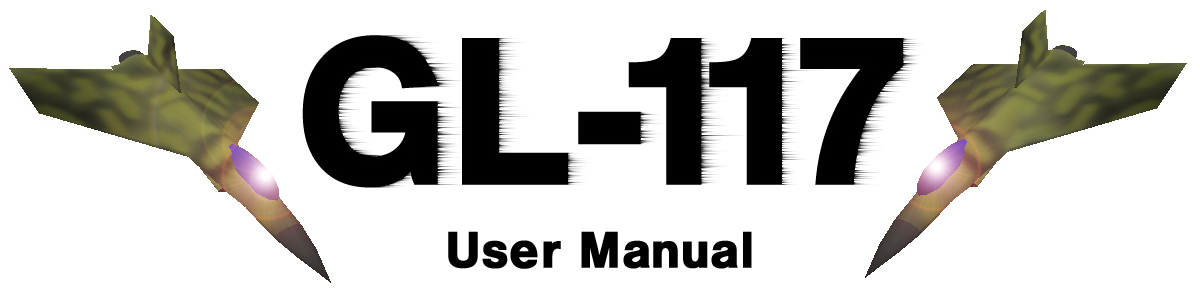
\includegraphics[width=16cm]{gl-117.jpg}
\end{center}

\vspace*{5cm}

\begin{center}
\Huge{User Manual}
\end{center}


%==============================================================================
% Preface/Table of contents
%==============================================================================
\pdfbookmark{Table of Contents}{toc}
\tableofcontents

% \pdfbookmark{List of Figures}{lof}
% \listoffigures

%==============================================================================
% Main part
%==============================================================================
\chapter{GL-117 Installation}
\label{chap:installation}

This chapter describes the requirements of \emph{GL-117} and its installation
concerning esp. the libraries required to compile and execute the game.

\section{Requirements}
\label{sec:requirements}

\emph{GL-117} requires Linux/Unix or MSWindows as operating system as well as
properly installed versions of the following libraries:
\begin{itemize}
\item{OpenGL or MesaGL: graphics library, 3D engine}
\item{GLU or MesaGLU: utilities for GL}
\item{GLUT or MesaGLUT: a toolkit that provides keyboard and mouse support}
\item{SDL (optional): the Direct Media Layer library has similar features of GLUT plus joystick
support and basic sound processing}
\item{SDL\_mixer (optional): a library that provides advanced multichannel sound
support and music}
\end{itemize}

Installation of \texttt{SDL} is optional, however strongly recommended.

\section{Downloading GL-117}
\label{sec:downloading_gl117}

The latest \emph{GL-117} release is currently available for download at
\texttt{http://www.freshmeat.net/gl-117} in \texttt{.tar.gz} and \texttt{.zip} format.
Using MSWindows you may prefer the \texttt{.zip} file that may be unpacked with
lots of programs like \texttt{PKUnzip, Winzip, WinRAR, WinACE}.
The \texttt{.tar.gz} version can be unpacked with GNU Tar using \\\texttt{tar xvfz
gl-117-x.y.z.tar.gz}\\ where \texttt{x.y.z} is the \emph{GL-117} version
number. For last minute updates and release-specific building and
install instructions, make sure to have a look at the
\texttt{README} and \texttt{INSTALL} files.

\section{Linux/Unix installation}
\label{sec:linux_installation}

If you got a binary \texttt{gl-117} in the \texttt{linux} directory, you will only
need the libraries \texttt{GL, GLU, GLUT} and \texttt{SDL, SDL\_mixer} as
described above.

In order to compile \emph{GL-117} you will also have to install the developement
versions of the libraries above (except \texttt{SDL\_mixer}).
To compile \emph{GL-117} do the following steps in the gl-117-\textit{VERSION}
directory:
\begin{verbatim}
 ./configure
 make
\end{verbatim}

The \texttt{configure} script will check for the required libraries and will output
a \texttt{Makefile}, which can be invoked using the \texttt{make} command.
After compiling \emph{GL-117} successfully, you will find a binary called \texttt{gl-117}
in the \texttt{src} directory. Move it to the \texttt{linux} directory manually and
execute.\\
To really install \emph{GL-117} please use:
\begin{verbatim}
 make install
\end{verbatim}
This will copy the binary to your binary directory (e.g. \texttt{/usr/local/bin})
and the rest of data files to your data directory (e.g. \texttt{/usr/local/share}).
Any files that require output permissions will be stored in the user's home directory,
exactly \texttt{\$HOME/.gl-117}.\\
This step will require write permissions in the binary and data directories.
However you may customize these directories using for example
\begin{verbatim}
 ./configure --prefix='/home/tom/gl-117'
 make
 make install
\end{verbatim}


\section{MSWindows installation}
\label{sec:windows_installation}

First, you might have to install \texttt{GL, GLU, GLUT} and \texttt{SDL, SDL\_mixer}.
Look into your system directory, that is generally
\begin{verbatim}
 \WINDOWS\SYSTEM    for Windows9x/ME
 \WINDOWS\SYSTEM32  for WindowsNT/2000/XP
\end{verbatim}
You will need the files \texttt{opengl32.dll, glu32.dll, glut32.dll, sdl.dll, sdl\_mixer.dll}
there.
If one is missing, please search the internet.
That's it. Execute the binary \texttt{gl-117.exe} in \emph{GL-117}'s \texttt{windows}
directory.\\

If you had already an earlier version of \emph{GL-117} you might want to use your
old pilots with the new version of the game. Therefore simply copy the old
\texttt{saves} directory to the new version.


\section{Running GL-117}
\label{sec:running_gl117}

At startup, \emph{GL-117} tries to read a file \texttt{conf} from the user's home
directory (Linux/Unix) or the \texttt{saves} directory (MSWindows).
If there is none, the game will try out some screen settings and store the file.
\begin{verbatim}
 Linux/Unix      $HOME/.gl-117/conf
 MSWindows       GL-117-INSTALLDIR/saves/conf
\end{verbatim}

Edit the file using your favourite text editor and adjust the settings
to your system.
If you lack a hardware accelerated video card, please turn down the
quality to 0 or 1. Further acceleration can be achieved negligating fullscreen mode
and choosing a lower resolution.\\
Just delete the \texttt{conf} file if you want to reset to the initial settings.

\chapter{GL-117 Aerodynamics}
\label{chap:aerodynamics}

This chapter gives a brief introduction on all the physics
a pilot has to consider when flying an aircraft.

\section{The four forces}
\label{sec:forces}

During flight the four forces acting on an aircraft are \textit{lift},
\textit{drag}, \textit{thrust}, and \textit{weight}, see fig \ref{fig:forces}.

\textit{Lift} is the upward force created by the airflow as it
passes over the wings.
In straight, unaccelerated flight, the lift compensates the
\textit{weight force} and therefore, the aircraft does not climb or dive.
The lifting force depends on the speed: low speed will cause the
airplane to dive, at high speed it will even climb.
Always consider the lift vector. If you fly a roll, the lift will not
oppose the weight any more and thus, you will lose height.

\textit{Drag} is the retarding force that limits the aircraft's speed.
There are many factors effecting drag, but one main cause
is simply the airplane's structure that protrudes into the wind.

\textit{Thrust} is the forward force provided by the engines.

Adding these four forces shows us how the speed of the fighter will change in the
next few seconds. The overall force is measured in G's with 1G meaning the
earth's gravity (about $9.81 m/s^2$). Pilots are often exposed to more than 1G, but
there are clearly limits: high forces above 9G may lead to a blackout and worse,
forces below -3G let the blood shoot into the head.

\emph{GL-117} provides two models: a simplified aerodynamics model making
it much easier to handle the aircraft thus promising more action
and a simulation model considering all the physical aspects as described above.

\begin{figure}
\begin{center}
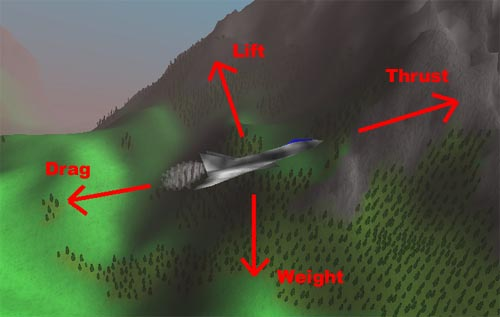
\includegraphics[width=10cm]{forces.jpg}
\caption{The four forces}
\label{fig:forces}
\end{center}
\end{figure}



\section{Three rotation axes}
\label{sec:axis}

All maneuvering takes place around three axes of rotation.
One way to define these axes is a carthesian coordinate system
with an x axis from left to right,
a y-axis from top to bottom, and a z-axis from near to far.
Imagine a flat landscape resembling the x-z plane.
Your viewing angle within this plane is called the \textit{heading},
whereas an orthogonal angle is called the \textit{elevation}.
Just look at figure \ref{fig:heading}.

But we can also define three axes of rotation referring to our fighter.
They are known as the \textit{longitudinal axis}, \textit{lateral axis},
and \textit{vertical axis}.
Imagine a coordinate system with the origin at your fighter's center of gravity.
The center of gravity is the theoretical point where the entire weight
of the aircraft is considered to be concentrated.

The \textit{lateral axis} is an imaginary axis protruding through the side
of the aircraft. A rotation around this axis is known as pitching.
This pitch movement is produced by the elevators and
will affect your heading and elevation.

The \textit{longitudinal axis} is an imaginary axis protruding through
the nose of the aircraft.
A rotation around this axis is known as a roll.
This roll movement is produced by the ailerons.
Consider that a roll will not change your heading.

The \textit{vertical axis} is an imaginary axis protruding through the top and
bottom
of the aircraft. A rotation around this axis is know as yawing.
This yaw movement is produced by the rudder.

Now, look at fig \ref{fig:fly}.
The blue arrows show the elevator's effect: your fighter will
either move up and left or it will drop down to the right
(the lateral axis).
Using the rudder will move the fighter slightly towards the green arrows
(the vertical axis).

\begin{figure}
\begin{tabular}{p{7.2cm}p{7.2cm}}
\begin{center}
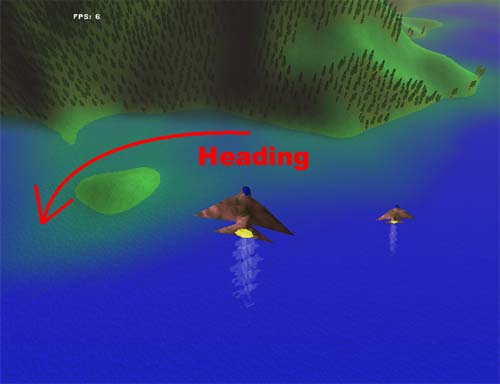
\includegraphics[width=7.2cm,height=6cm]{heading.jpg}
\label{fig:heading}
\end{center} &
\begin{center}
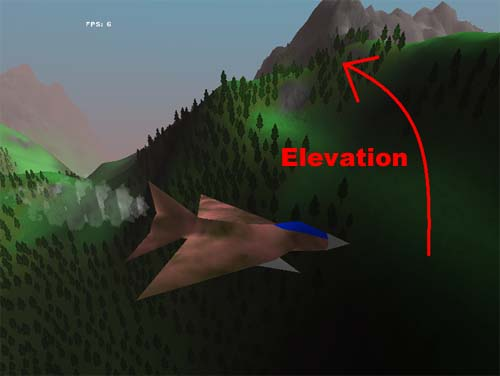
\includegraphics[width=7.2cm,height=6cm]{elevation.jpg}
\label{fig:elevation}
\end{center}\\
\begin{center}
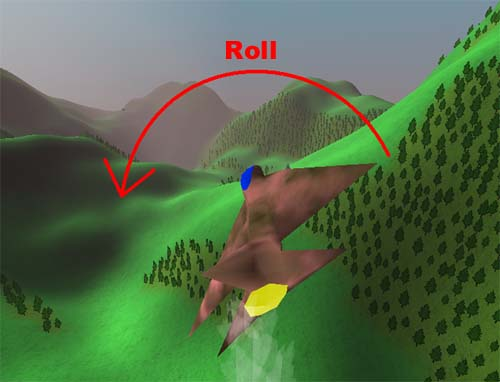
\includegraphics[width=7.2cm,height=6cm]{roll.jpg}
\label{fig:roll}
\end{center} &
\begin{center}
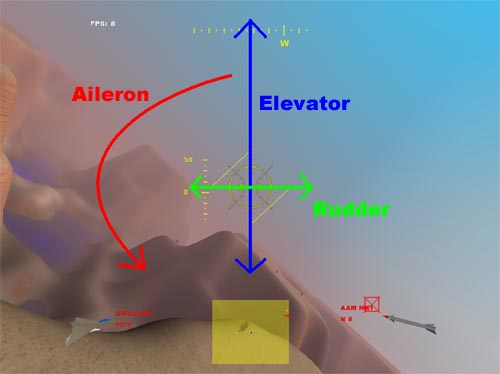
\includegraphics[width=7.2cm,height=6cm]{fly.jpg}
\label{fig:fly}\\
\end{center}
\end{tabular}
\caption{The three axes of rotation}
\end{figure}

\chapter{GL-117 Basics}
\label{chap:basics}

Having understood the physical aspects of piloting,
you may now get an introduction to the game itself.


\section{Cockpit controls}
\label{sec:cockpit}

\begin{figure}
\begin{center}
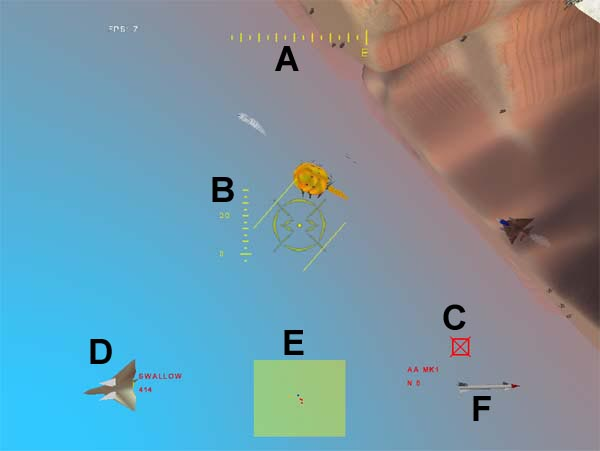
\includegraphics[width=12cm]{hud.jpg}
\caption{A typical HUD of GL-117}
\label{fig:hud}
\end{center}
\end{figure}

Figure \ref{fig:hud} shows a typical \textit{HUD} (head-up display):
\begin{itemize}
\item{A: your current heading, showing the letters \texttt{'N', 'E', 'S', W'}
to represent north, east, south, west.}
\item{B: your current elevation in degree; the rotating lines reveal the
horizon and thus your roll angle.}
\item{C: your current target}
\item{D: the radar reveals the position of other targets. Enemies are marked red,
allies blue. The screen is only 2D, so it will only reveal the necessary \textit{heading} to
other targets.}
\item{F: your currently selected weapon}
\item{G: the chaff/flare countermeasure systems alarms you about enemy missiles.}
\end{itemize}



\section{Input devices}
\label{sec:input_devices}

\emph{GL-117} supports a number of devices depending on \texttt{GLUT} and \texttt{SDL}.
You may choose your preferred input device within the options menu.
It is strongly recommended to use a joystick, however the mouse interface
is also very easy to handle.

\subsection{The keyboard}
\label{subsec:keyboard}

\begin{center}
\begin{tabular}{|c|c|l|l|l|}
\hline
\textsc{Key} & \textsc{Meaning}\\\hline
UP, DOWN & Elevator\\
LEFT, RIGHT & Roll\\
PAGEUP, PAGEDOWN & Rudder\\
1, 2, 3, 4, 5, 6, 7, 8, 9 & Throttle\\
\hline
SPACE & Fire cannon\\
m & Change weapon/missile\\
ENTER & Fire weapon/missile\\
\hline
t & Target next object\\
e & Target nearest enemy\\
\hline
ESC & Main menu\\
\hline
F1 & Cockpit camera\\
F2 & Chase camera\\
F3 & Rear camera\\
F4, F5 & Side cameras\\
F6, F7, F8 & Top cameras\\
\hline
\end{tabular}
\end{center}

Note that the tabular only shows the predefined settings. You may customize the
keyboard editing the file \texttt{conf.interface} located in the \texttt{saves}
directory on MSWindows, in the directory \texttt{\$HOME/.gl-117} for UNIX respectively.


\subsection{The mouse}
\label{subsec:mouse}

Moving the mouse up or down will change the elevator to fly a loop, whereas
moving left or right will result in a roll, a slight movement will
affect the rudder.\\
To change your heading, you will thus have to move the mouse cursor completely
to the left/right for a short moment (just figure it out) in order to fly a
quarter roll. Return the mouse cursor to the center immediately!
Then alter the elevator moving the mouse to the top center of your screen to
fly a "loop" parallel to the surface.\\
The left mouse button can be used to fire the cannon, the right button will
fire the weapon/missile, although it is recommended to use the keyboard for
targeting and firing purpose.\\
Look at the keyboard table for a list of keys.\\
Along with the "mouse easy" interface comes the possibility to revert the
elevator controls, called "mouse reverse". Only experienced players should
use this option.


\subsection{The joystick}
\label{subsec:joystick}

The easiest interface to play \emph{GL-117} is likely the joystick.\\
\emph{GL-117} supports up to four joystick axes:
moving the joystick up or down will change the elevator, moving left or right
will affect the aileron, turning the joystick along the rudder will alter
the fighter's rudder settings, and moving the throttle will change
the fighter's throttle. If two axes functions are swapped, please edit the file
\texttt{conf.interface} to correct the settings.\\\\
Depending on your joystick, \emph{GL-117} supports four buttons:
fire cannon, target nearest enemy, change weapon/missile, fire weapon/missile.\\\\
Any properly installed joystick will be available automatically.


\section{The menu}
\label{sec:menu}

As the menu is almost completely self-explanatory, there is only a brief
description of the different menu items:
\begin{itemize}
\item{The \texttt{PILOTS} menu lets you create and delete pilots. You can
play only one pilot at a time.}
\item{The \texttt{MISSIONS} menu shows all available missions. You have to
succeed in a mission to enable the next one.
Every mission you succeed will earn you a certain score, being calculated
depending on the time it took, the shield you lost, how many targets you
eliminated, and a difficulty bonus.
High scores are necessary to get a promotion to a higher military rank.
The difficulty bonus is added to the overall score automatically.}
\item{Several \texttt{OPTIONS} may be adjusted: quality, view, sound, music,
difficulty.}
\end{itemize}

To get the best graphics possible on your system, always look at the
\texttt{FPS} rate which describes the number of frames per second.
This rate is directly influenced by the quality and view settings and
should not drop below 25. If your rate is above 50 FPS, you should
use higher/better quality and view settings.
You should also try out higher screen resolutions modifying the file
\texttt{conf} located in the \texttt{saves}
directory on MSWindows, in the directory \texttt{\$HOME/.gl-117} for UNIX respectively.

\chapter{The Eagle Squad}
\label{chap:squad}

You will fly missions for the Eagle Squad, which
is known for a good equipment and the best pilots.
Just look at the fighter and pilot overviews.


\section{The Fighters}
\label{sec:fighters}

\begin{center}
\begin{tabular}{|c|l|}
\hline
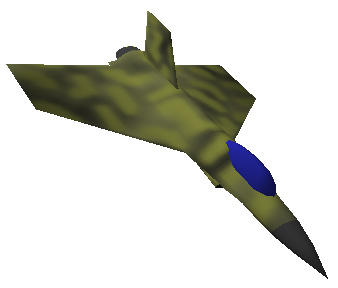
\includegraphics[width=4cm]{falcon.jpg} &
The GL-16 Falcon is an advanced fighter of the Eagle squadron.\\
\hline
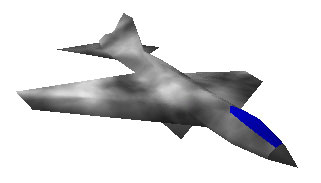
\includegraphics[width=4cm]{crow.jpg} &
The Crow is a typical enemy fighter.\\
\hline
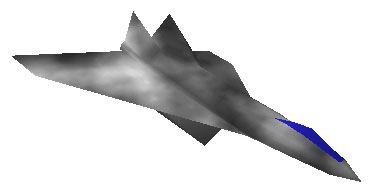
\includegraphics[width=4cm]{hawk.jpg} &
The GL-22 Hawk is the Red Eagle's bomber.\\
\hline
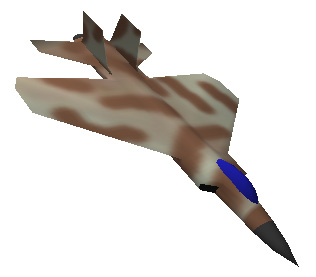
\includegraphics[width=4cm]{swallow.jpg} &
The Swallow is an advanced enemy bomber.\\
\hline
\end{tabular}
\end{center}


\section{The Weapons}
\label{sec:weapons}

\begin{center}
\begin{tabular}{|c|l|}
\hline
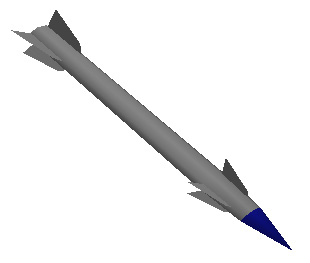
\includegraphics[width=3cm]{missile_ff.jpg} &
The FF is a radar controlled friend-foe air-air missile.\\
\hline
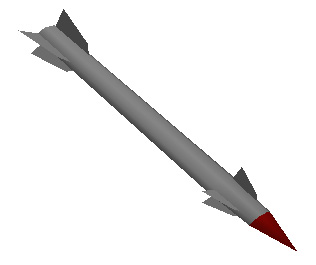
\includegraphics[width=3cm]{missile_ir.jpg} &
The IR is an infra red air-air missile.\\
\hline
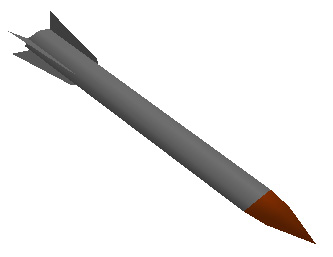
\includegraphics[width=3cm]{missile_agm.jpg} &
The AGM is a medium air-ground missile.\\
\hline
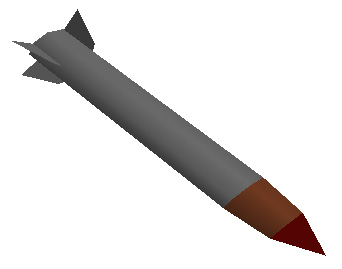
\includegraphics[width=3cm]{missile_df.jpg} &
The DF is an uncontrolled dumb fire missile.\\
\hline
\end{tabular}
\end{center}

Use FF missiles early when approaching the enemy.
They will search their target using a radar system,
however a chaff cloud may fool them.

IR missiles can only track the enemy by heat and must
therefore be fired at the enemy's back.
Flares consisting of burning magnesium can be used as a countermeasure.

AGMs are radar controlled missiles used to
take out medium ground targets like tanks.

DF missiles will only fly straight ahead like cannon shots,
but can cause an enormous amount of damage,
so they are used to take out huge ground targets like buildings.


%==============================================================================
% Appendix
%==============================================================================
\appendix
% \input{quotes}
% \input{glossary}

%==============================================================================
% Bibliography/ Index
%==============================================================================
% comment the next line not to cite ALL BiBTeX entries
% \nocite{*}
% \pdfbookmark{Bibliography}{bibliography}
% \bibliography{sep}

\end{document}

